\begin{frame}{数值算例}
    \begin{columns}
        \column{0.35\textwidth}
            \begin{figure}
                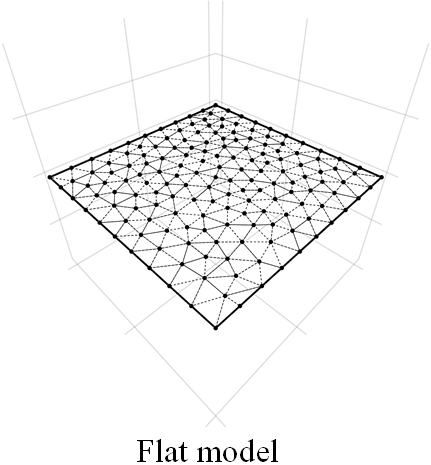
\includegraphics[width=\linewidth, trim=10 0 10 0, clip]{figures/ptmsh1.png}
            \end{figure}

        \column{0.65\textwidth}
            \begin{table}[!ht]
            \centering
            \footnotesize
            \caption{Results of patch test for flat model.}
            \begin{tabular}{lcccc}
            \toprule
            & \multicolumn{2}{c}{Linear patch test} & \multicolumn{2}{c}{Quadratic patch test} \\ \cline{2-5}
            & $L_2$-Error & $H_e$-Error & $L_2$-Error & $H_e$-Error \\
            \midrule
            GI-Penalty & 1.41E-04 & 4.62E-03 & 1.97E-03 & 7.17E-03 \\
            GI-Nitsche & 1.73E-04 & 5.61E-03 & 1.85E-03 & 7.76E-03 \\
            RKGSI-Penalty & 5.04E-09 & 1.02E-07 & 3.01E-09 & 3.41E-08 \\
            RKGSI-Nitsche & 9.75E-12 & 8.98E-11 & 1.29E-12 & 1.06E-12 \\
            RKGSI-HR & 6.15E-13 & 6.91E-12 & 7.51E-13 & 8.36E-12 \\
            \bottomrule
            \end{tabular}
        \end{table}

        \vspace{0.1cm}
        \centering
        \footnotesize
        $\boldsymbol v = \begin{Bmatrix}
        (\xi^1+2\xi^2)^n \\ (3\xi^1+4\xi^2)^n \\ (5\xi^1+6\xi^2)^n
        \end{Bmatrix}$,\quad
        $n = \begin{cases}
        1 & \text{Linear} \\
        2 & \text{Quadratic}
        \end{cases}$
    \end{columns}
\end{frame}


\begin{frame}{数值算例}
    \begin{columns}
        \column{0.35\textwidth}
            \begin{figure}
                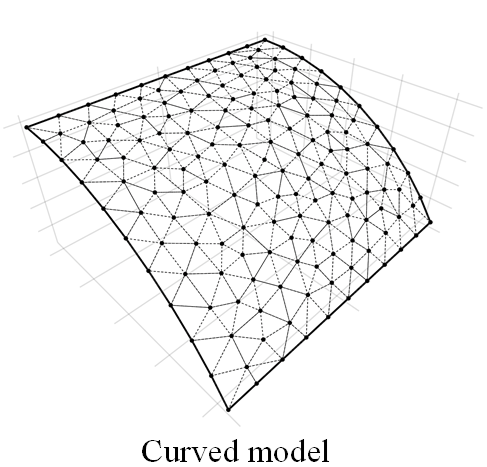
\includegraphics[width=\linewidth, trim=10 0 10 0, clip]{figures/ptmsh.png}
            \end{figure}

        \column{0.65\textwidth}
            \begin{table}[!ht]
            \footnotesize
            \centering
            \caption{Results of patch test for cylindrical model.}\label{ptt2}
            \begin{tabular}{lcccc}
            \toprule
            & \multicolumn{2}{c}{Linear patch test} & \multicolumn{2}{c}{Quadratic patch test} \\ \cline{2-5}
            & $L_2$-Error & $H_e$-Error & $L_2$-Error & $H_e$-Error \\
            \midrule
            GI-Penalty & 1.75E-04 & 4.50E-03 & 1.08E-03 & 5.83E-03 \\
            GI-Nitsche & 1.77E-04 & 5.36E-03 & 1.07E-03 & 6.33E-03 \\
            RKGSI-Penalty & 8.59E-05 & 9.11E-04 & 4.28E-04 & 2.08E-03 \\
            RKGSI-Nitsche & 1.27E-05 & 5.32E-05 & 1.88E-05 & 5.6E-04 \\
            RKGSI-HR & 1.43E-05 & 1.60E-04 & 2.93E-05 & 2.85E-04 \\
            \bottomrule
        \end{tabular}
        \end{table}

        \vspace{0.1cm}
        \centering
        \footnotesize
        $\boldsymbol v = \begin{Bmatrix}
        (\xi^1+2\xi^2)^n \\ (3\xi^1+4\xi^2)^n \\ (5\xi^1+6\xi^2)^n
        \end{Bmatrix}$,\quad
        $n = \begin{cases}
        1 & \text{Linear} \\
        2 & \text{Quadratic}
        \end{cases}$
    \end{columns}
\end{frame}

\begin{frame}{数值算例}
    \begin{columns}
        \column{0.35\textwidth}
            \begin{figure}
                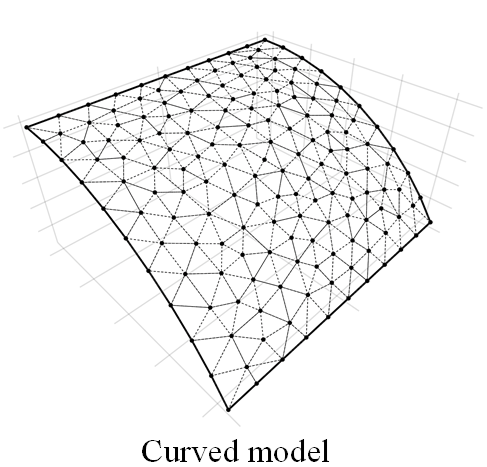
\includegraphics[width=\linewidth, trim=10 0 10 0, clip]{figures/ptmsh.png}
            \end{figure}
        \column{0.65\textwidth}
            \begin{figure}
                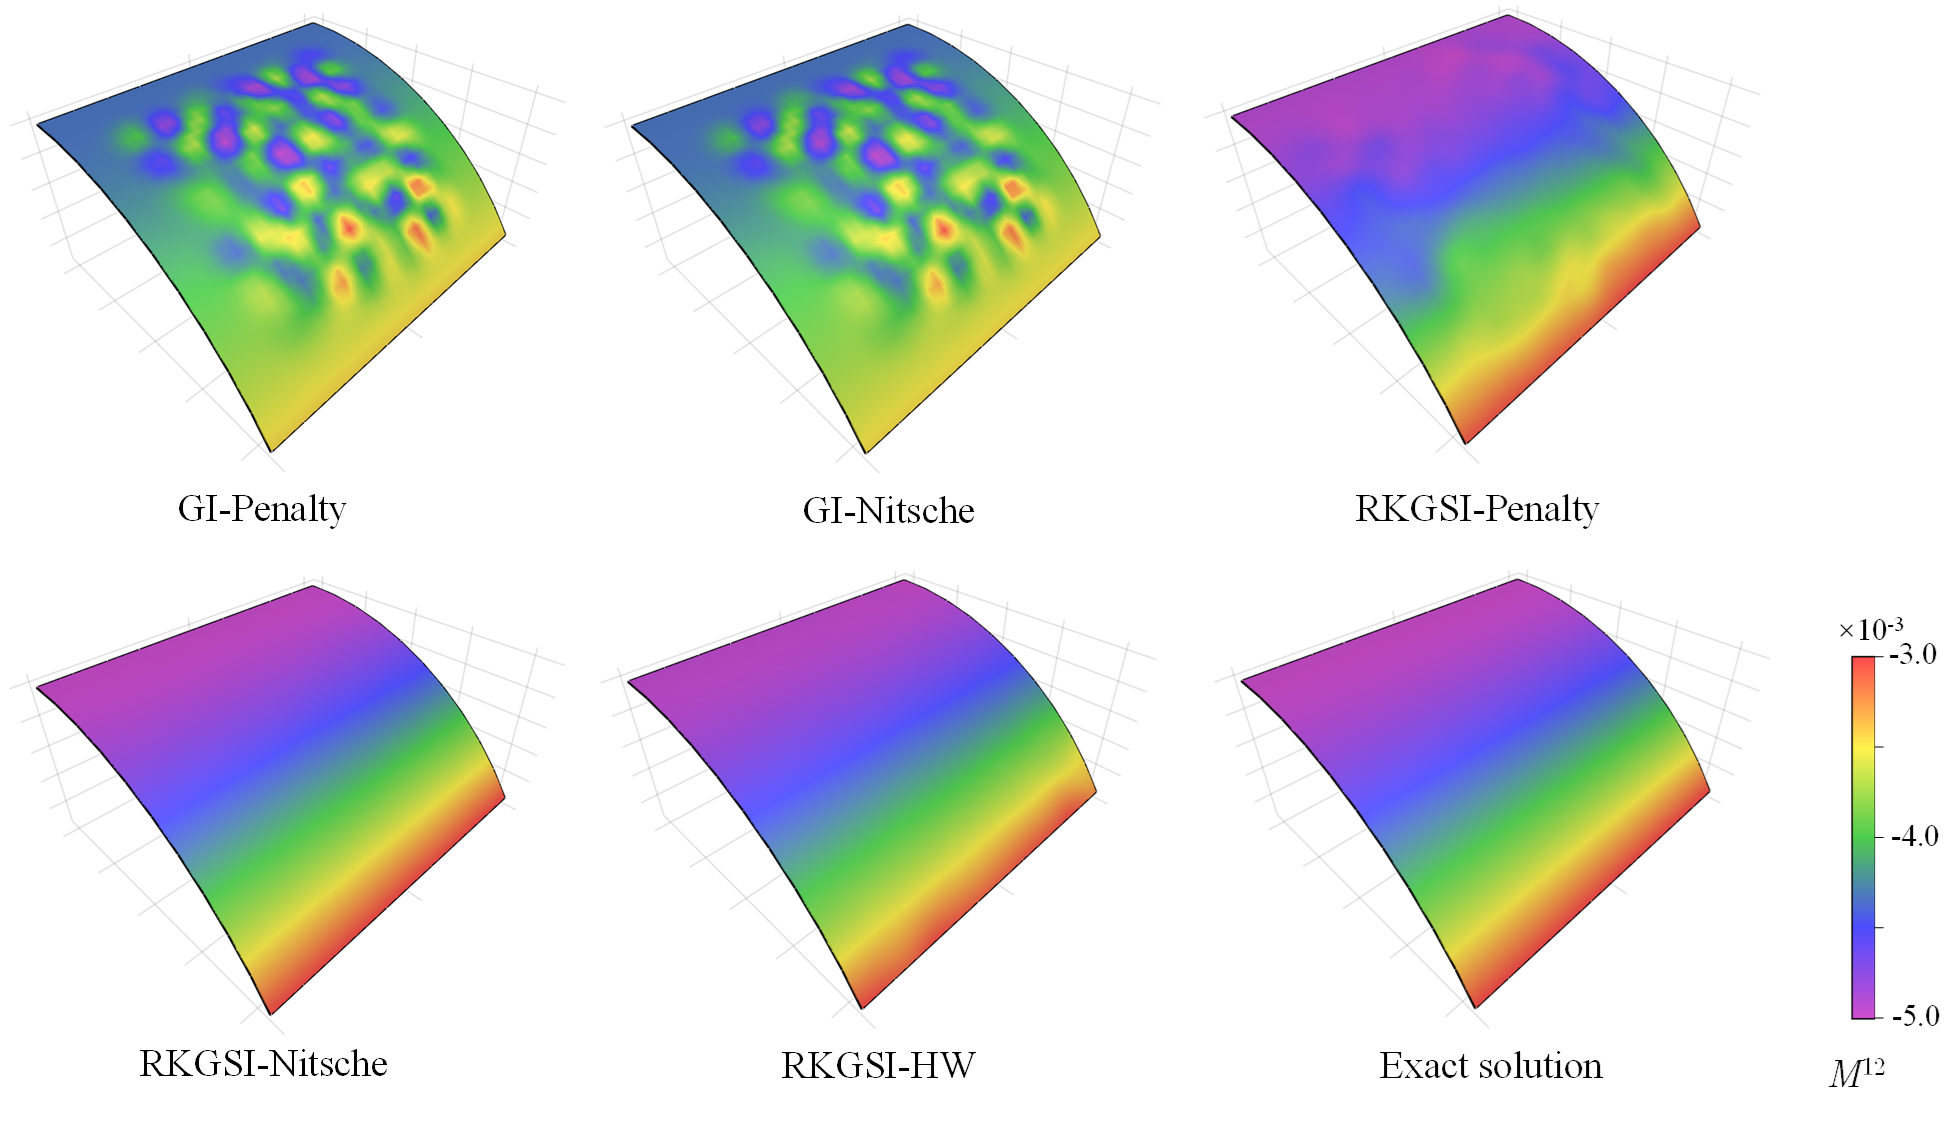
\includegraphics[width=\linewidth, trim=15 10 10 0, clip]{figures/ptc_r2.png}
                \caption{曲壳分片试验$M^{12}$云图}
            \end{figure}
    \end{columns}
\end{frame}

\begin{frame}{数值算例}
    \begin{columns}
        \column{0.4\textwidth}
            \begin{figure}
                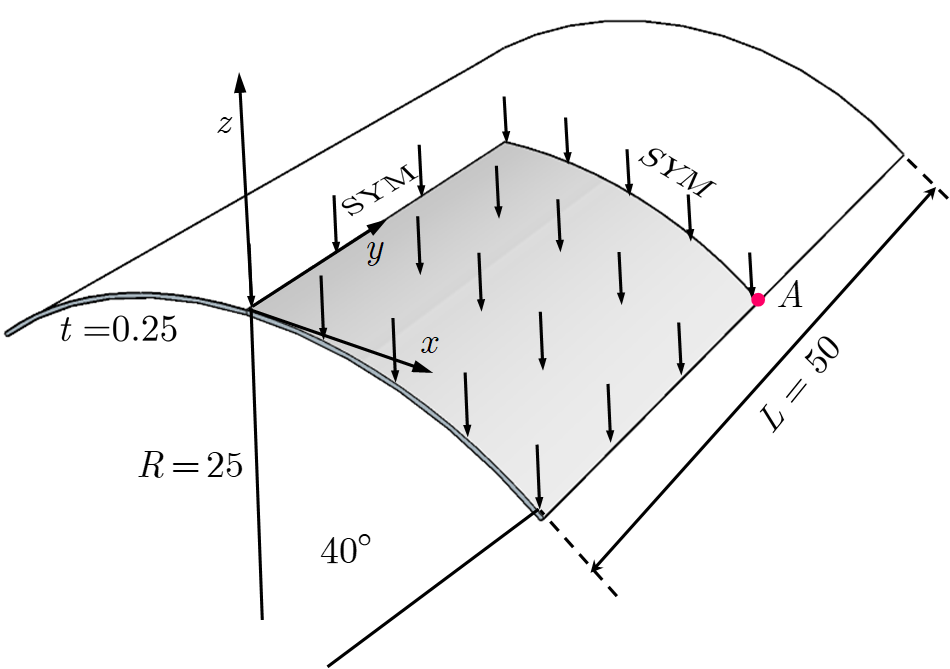
\includegraphics[height=0.7\textwidth]{figures/slm.png}
                \caption{Scordelis-Lo 屋顶问题描述}

                \centering
                \small
                {\color{myblue}
                \fbox{
                \begin{tabular}{@{} l @{\quad} l @{}}
                    \textbf{杨氏模量} & $E = 4.32 \times 10^8$ \\[0.8em]
                    \textbf{泊松比}   & $\nu = 0.0$           \\[0.8em]
                    \textbf{荷载}     & $q = 90.0$
                \end{tabular}
                }}
            \end{figure}
        \column{0.55\textwidth}
            \begin{figure}
                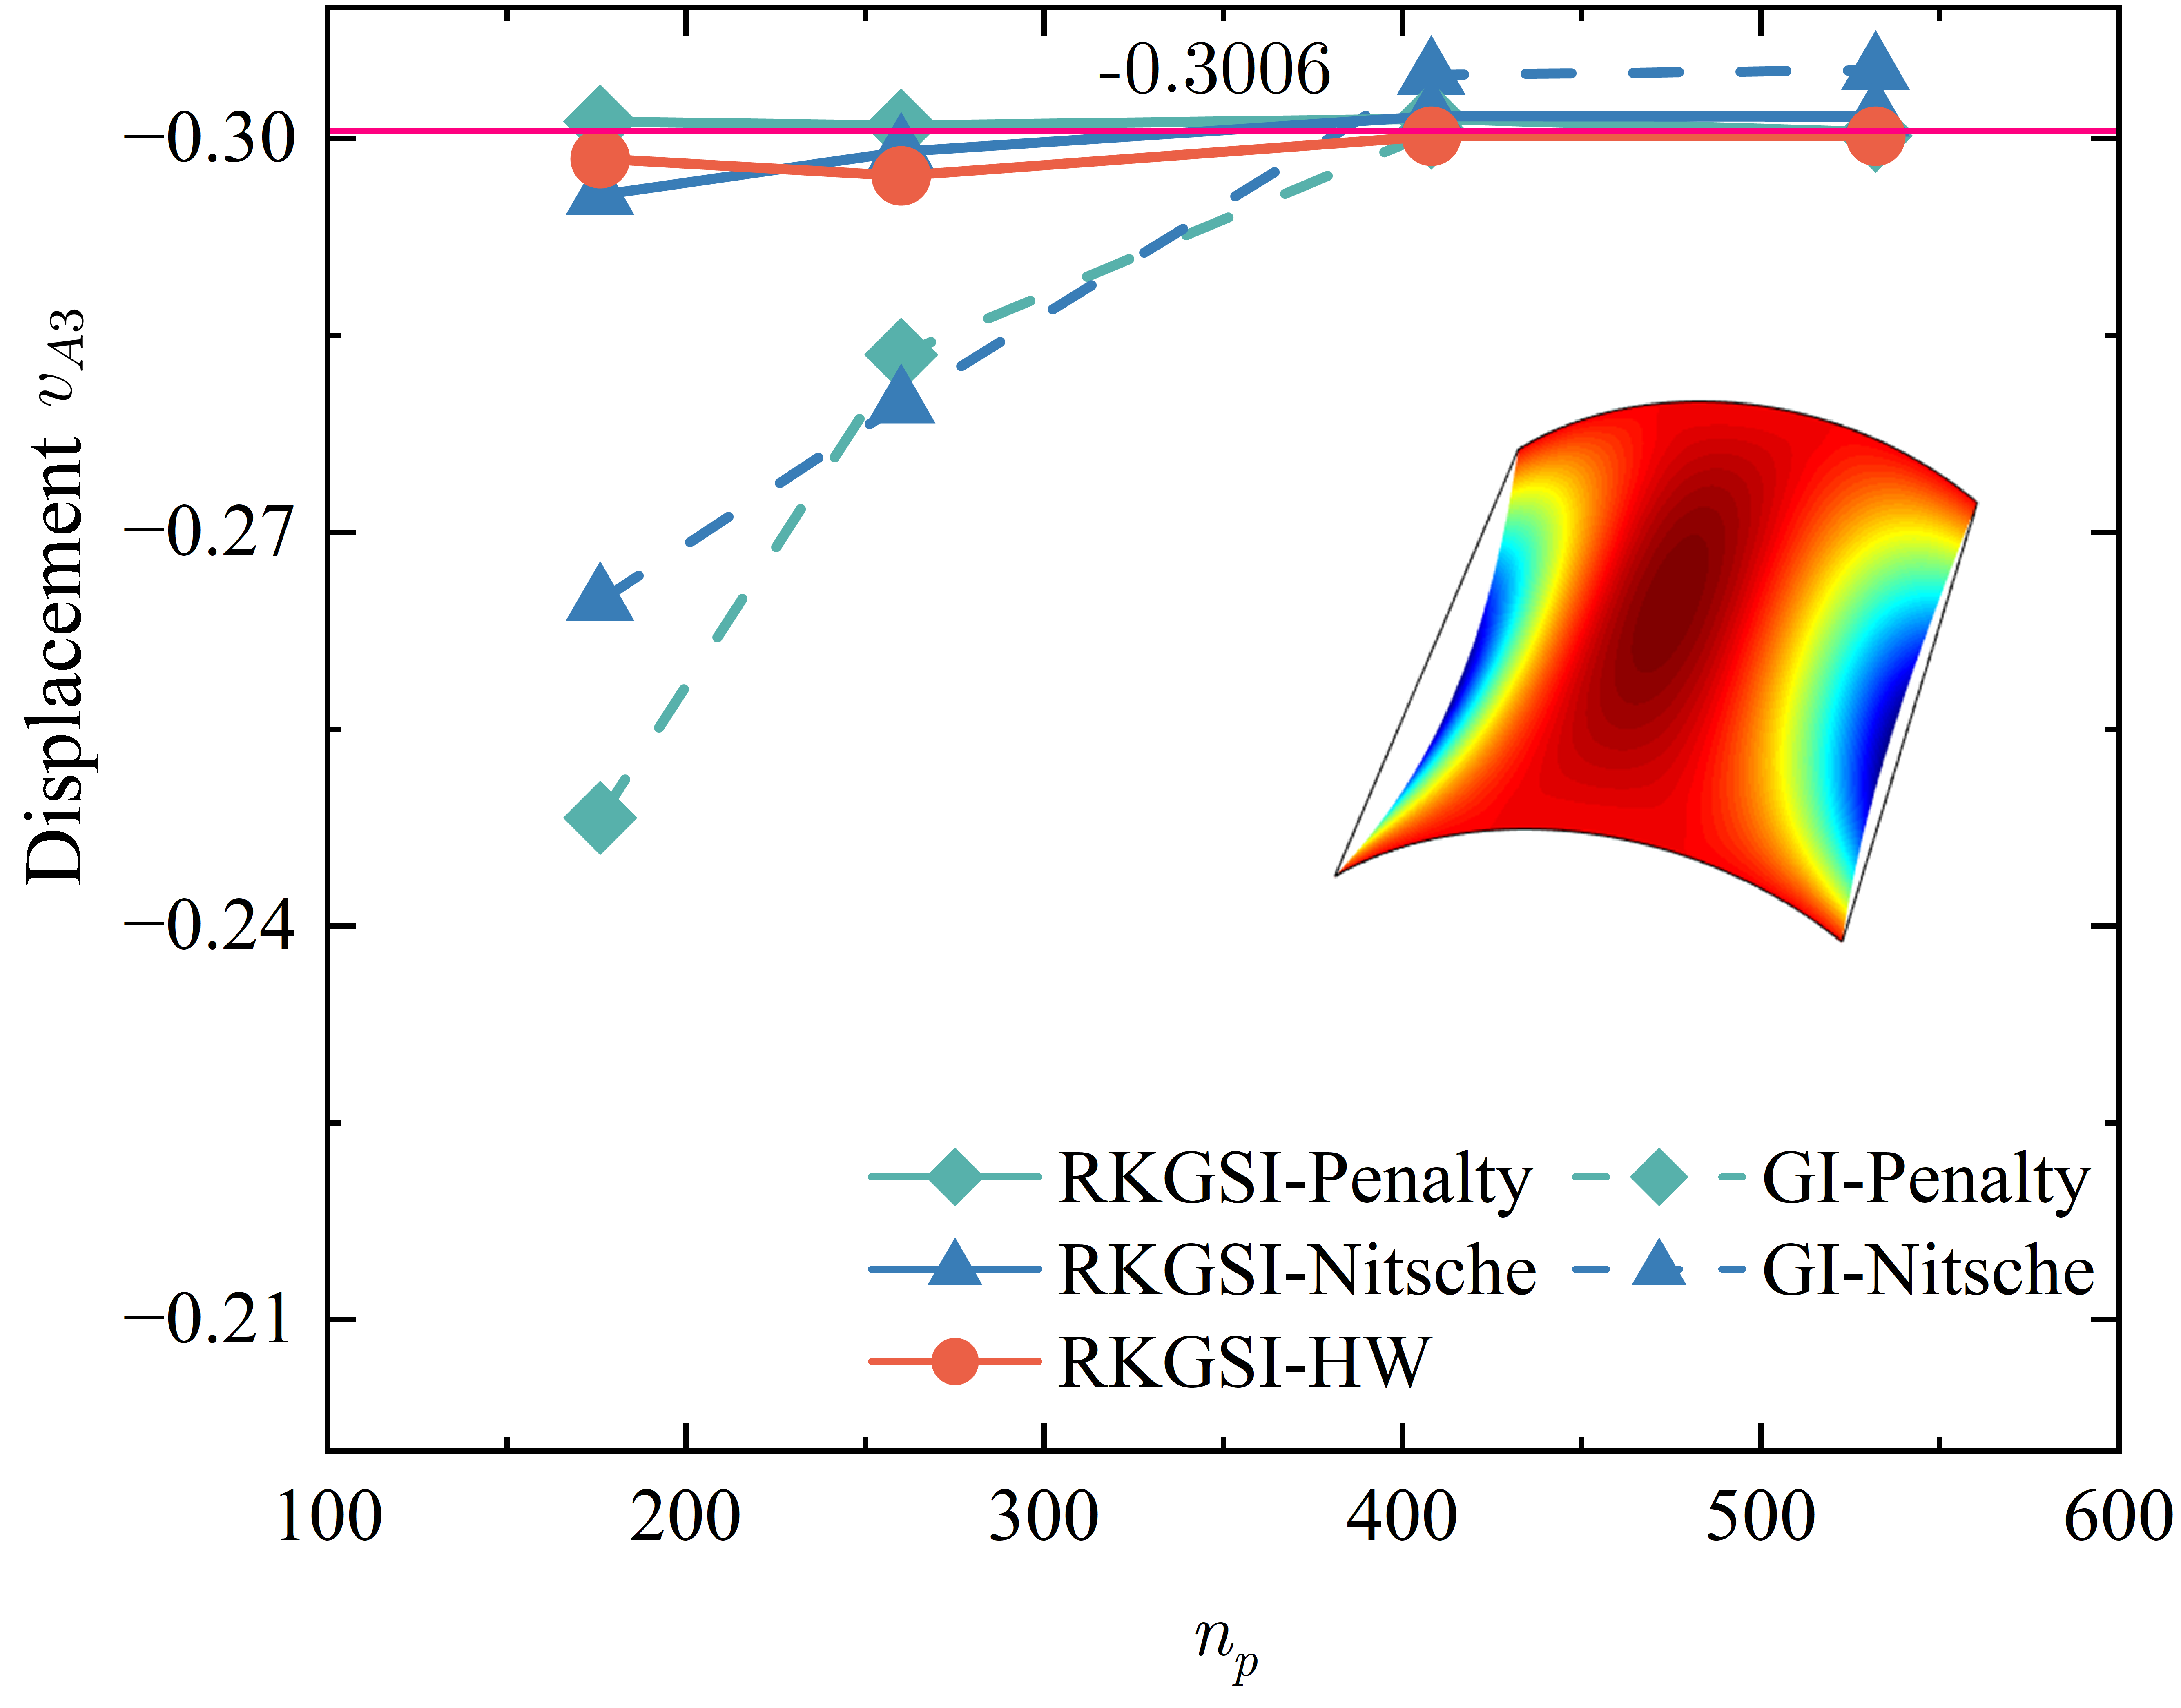
\includegraphics[height=0.7\textwidth]{figures/sld_r2.png}
                \caption{Scordelis-Lo屋顶问题的位移收敛性}
            \end{figure}
    \end{columns}
\end{frame}

\begin{frame}{数值算例}
\begin{figure}[htbp]
    \centering 
    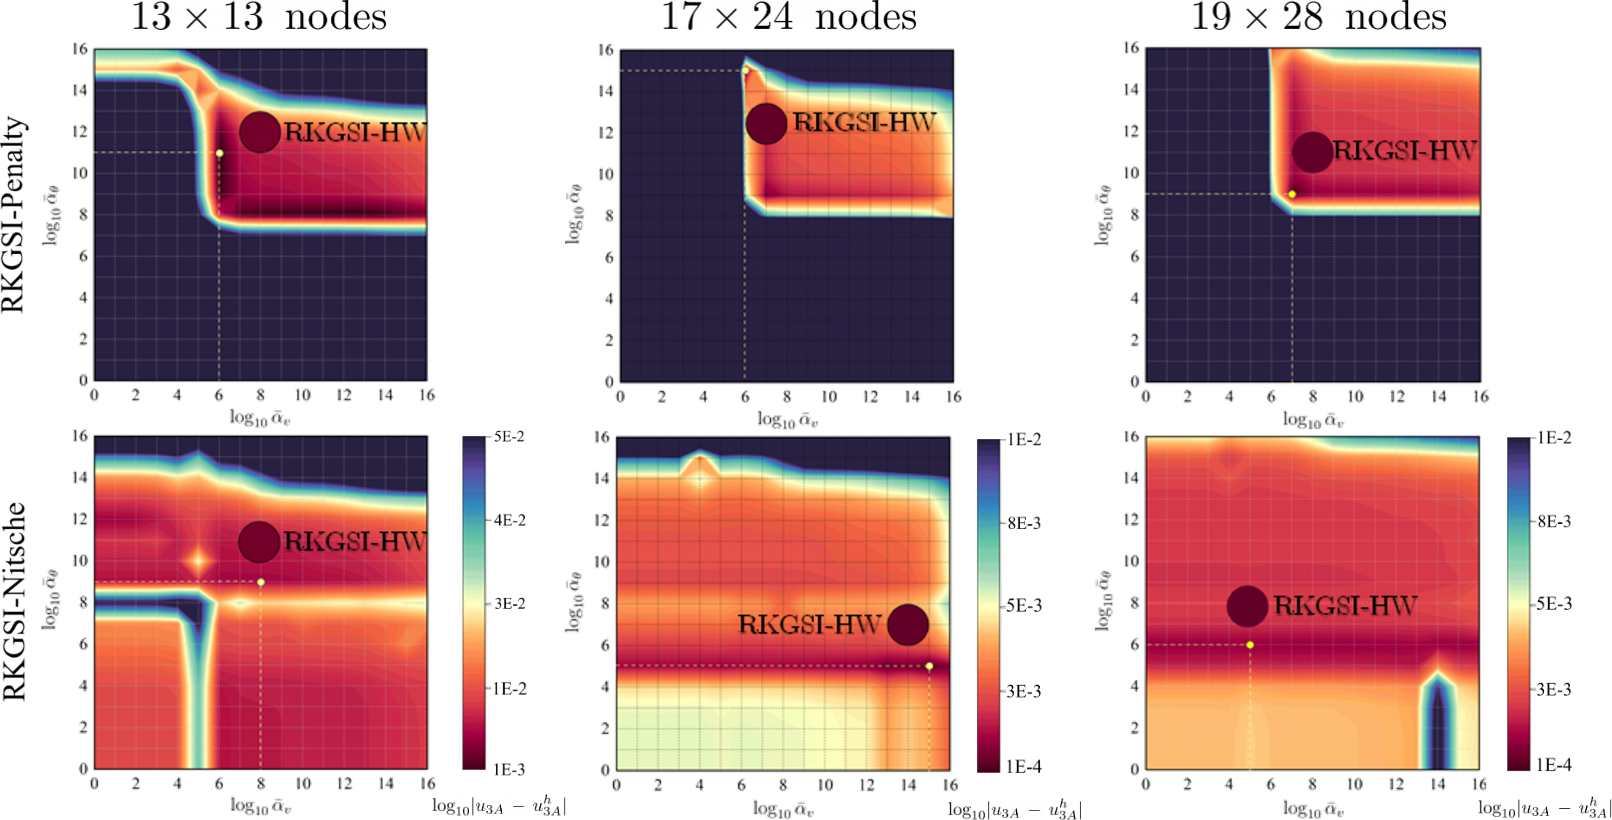
\includegraphics[width=0.85\textwidth]{figures/RKGSI.png}
    \caption{Scordelis‑Lo 屋顶问题中参数$\alpha_v$和$\alpha_\theta$的灵敏度对比}
\end{figure}
\end{frame}

\begin{frame}{数值算例}
    \begin{columns}
        \column{0.4\textwidth}
            \begin{figure}
                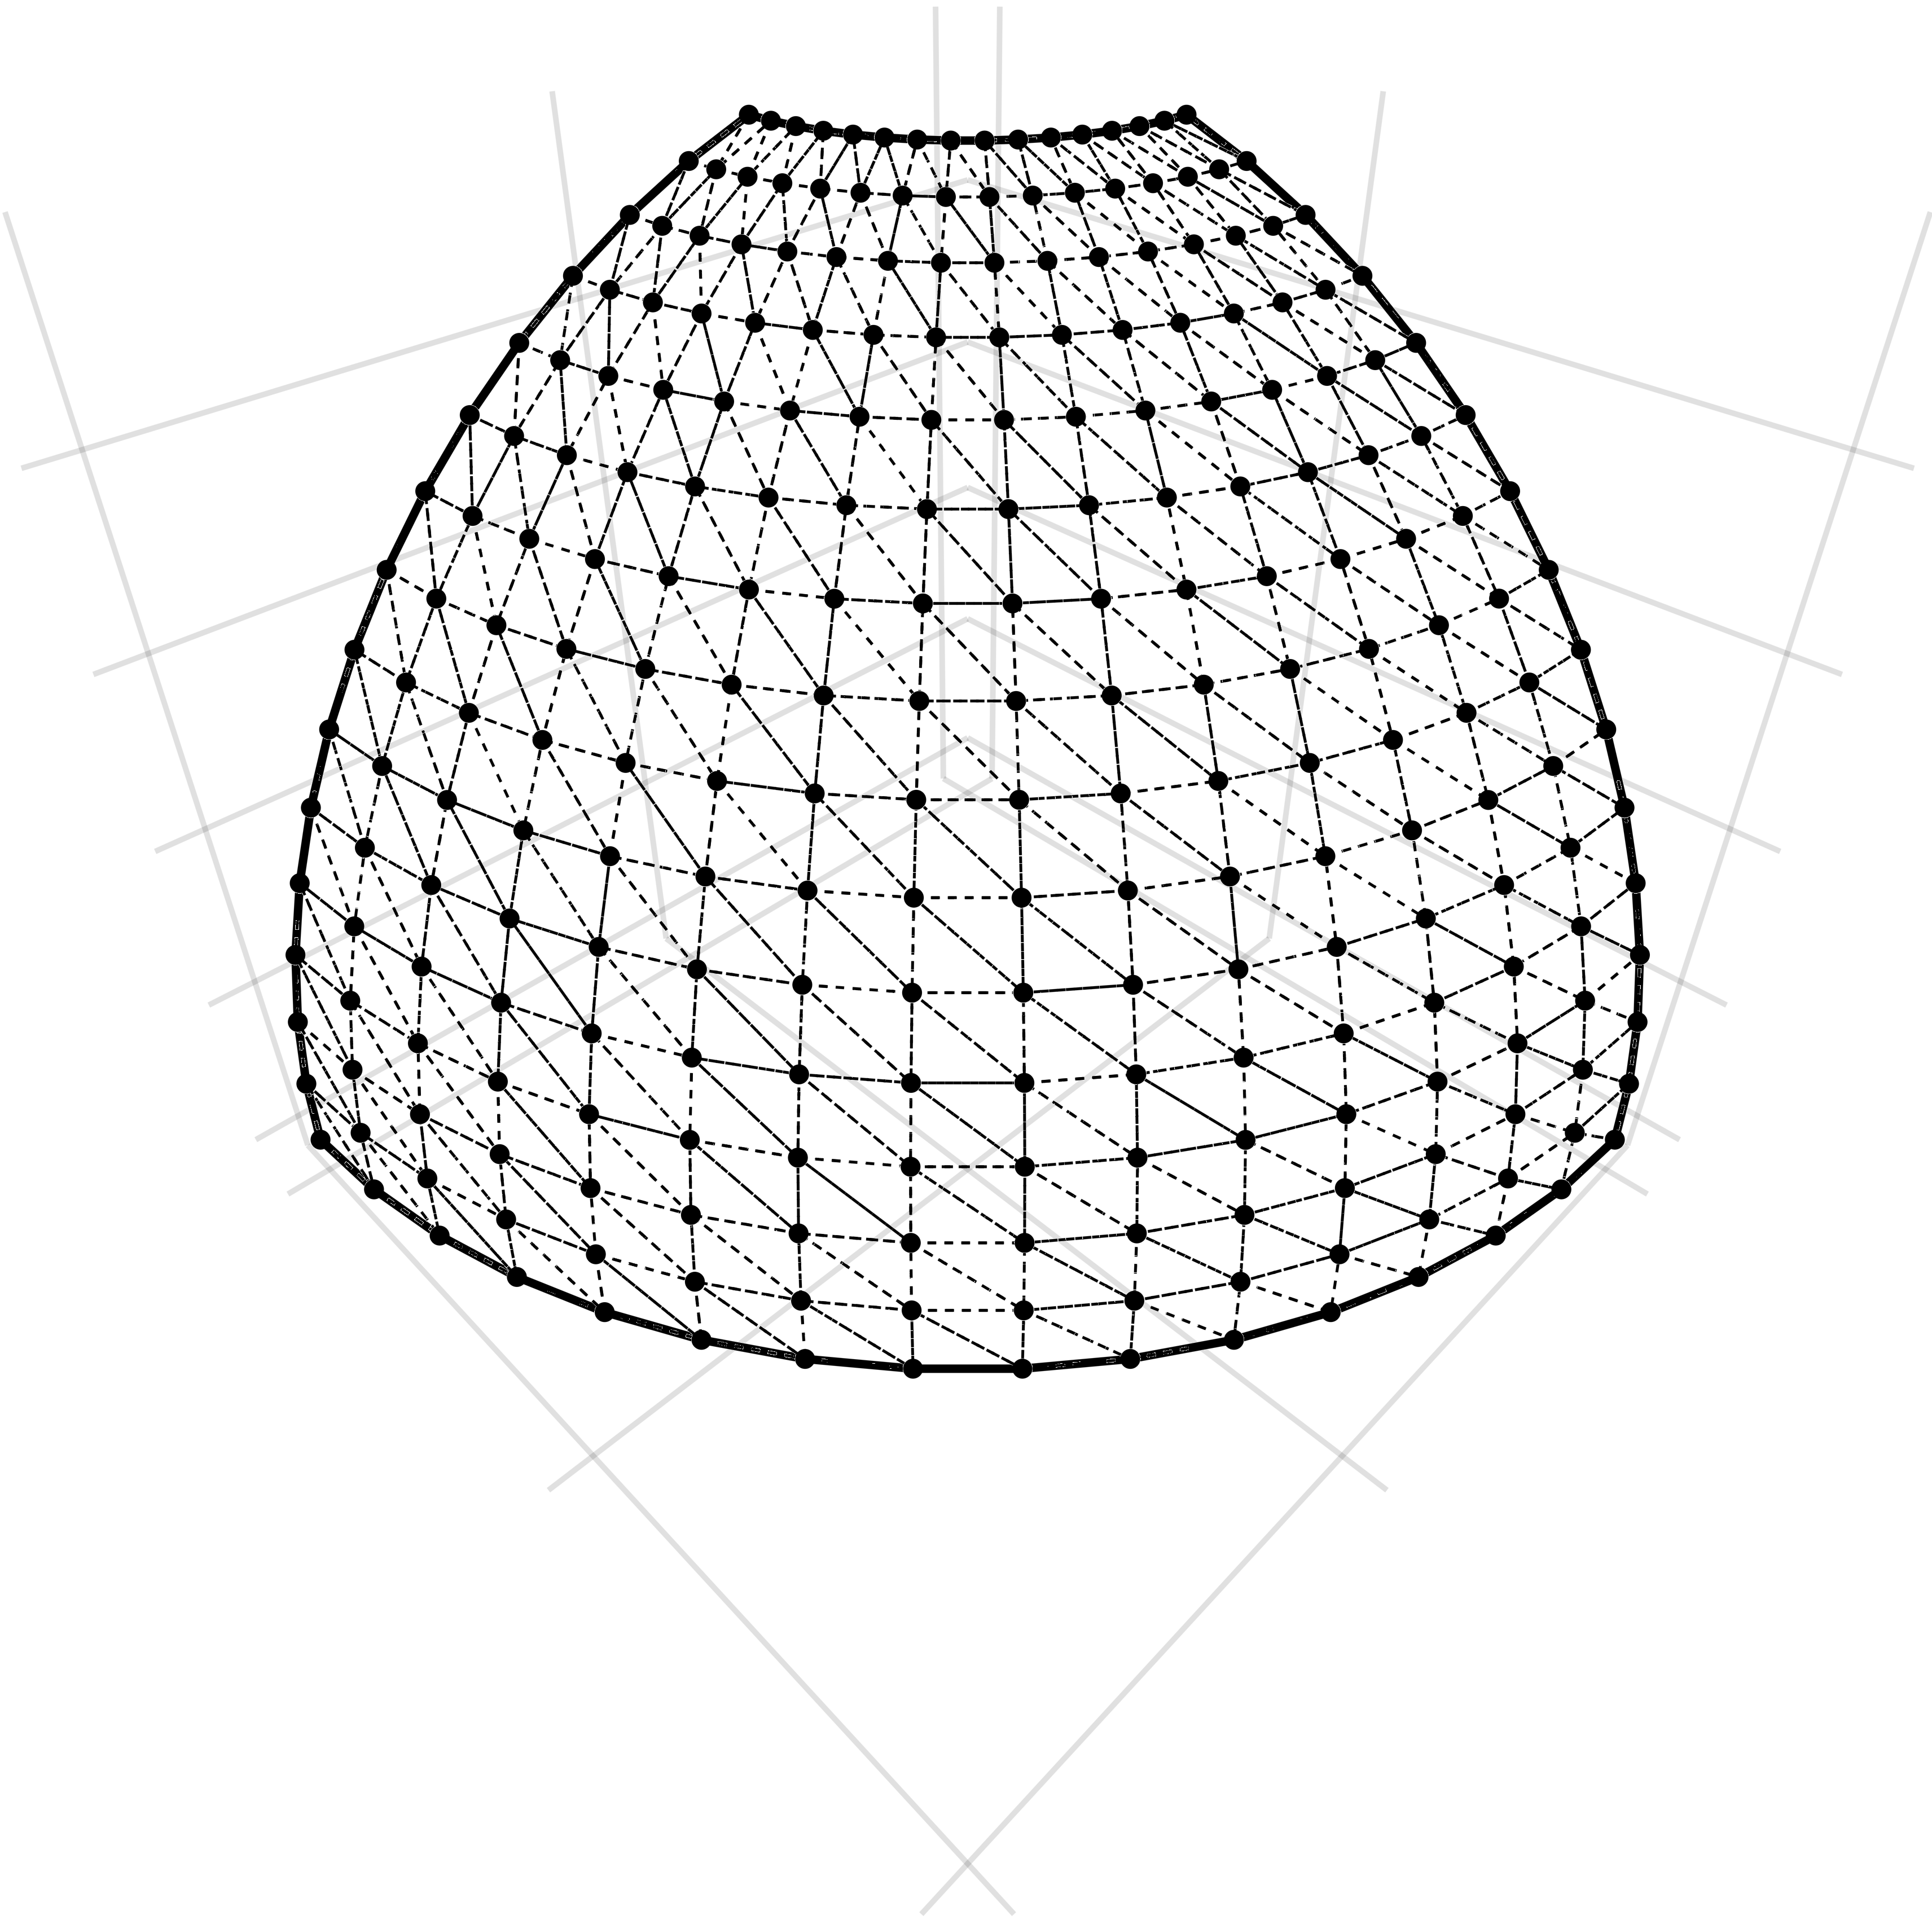
\includegraphics[width=\linewidth, trim=50 0 50 0, clip]{figures/sphericalshell_16.png}
                \caption{曲壳屋顶问题}
            \end{figure}
        \column{0.55\textwidth}
            \begin{figure}
                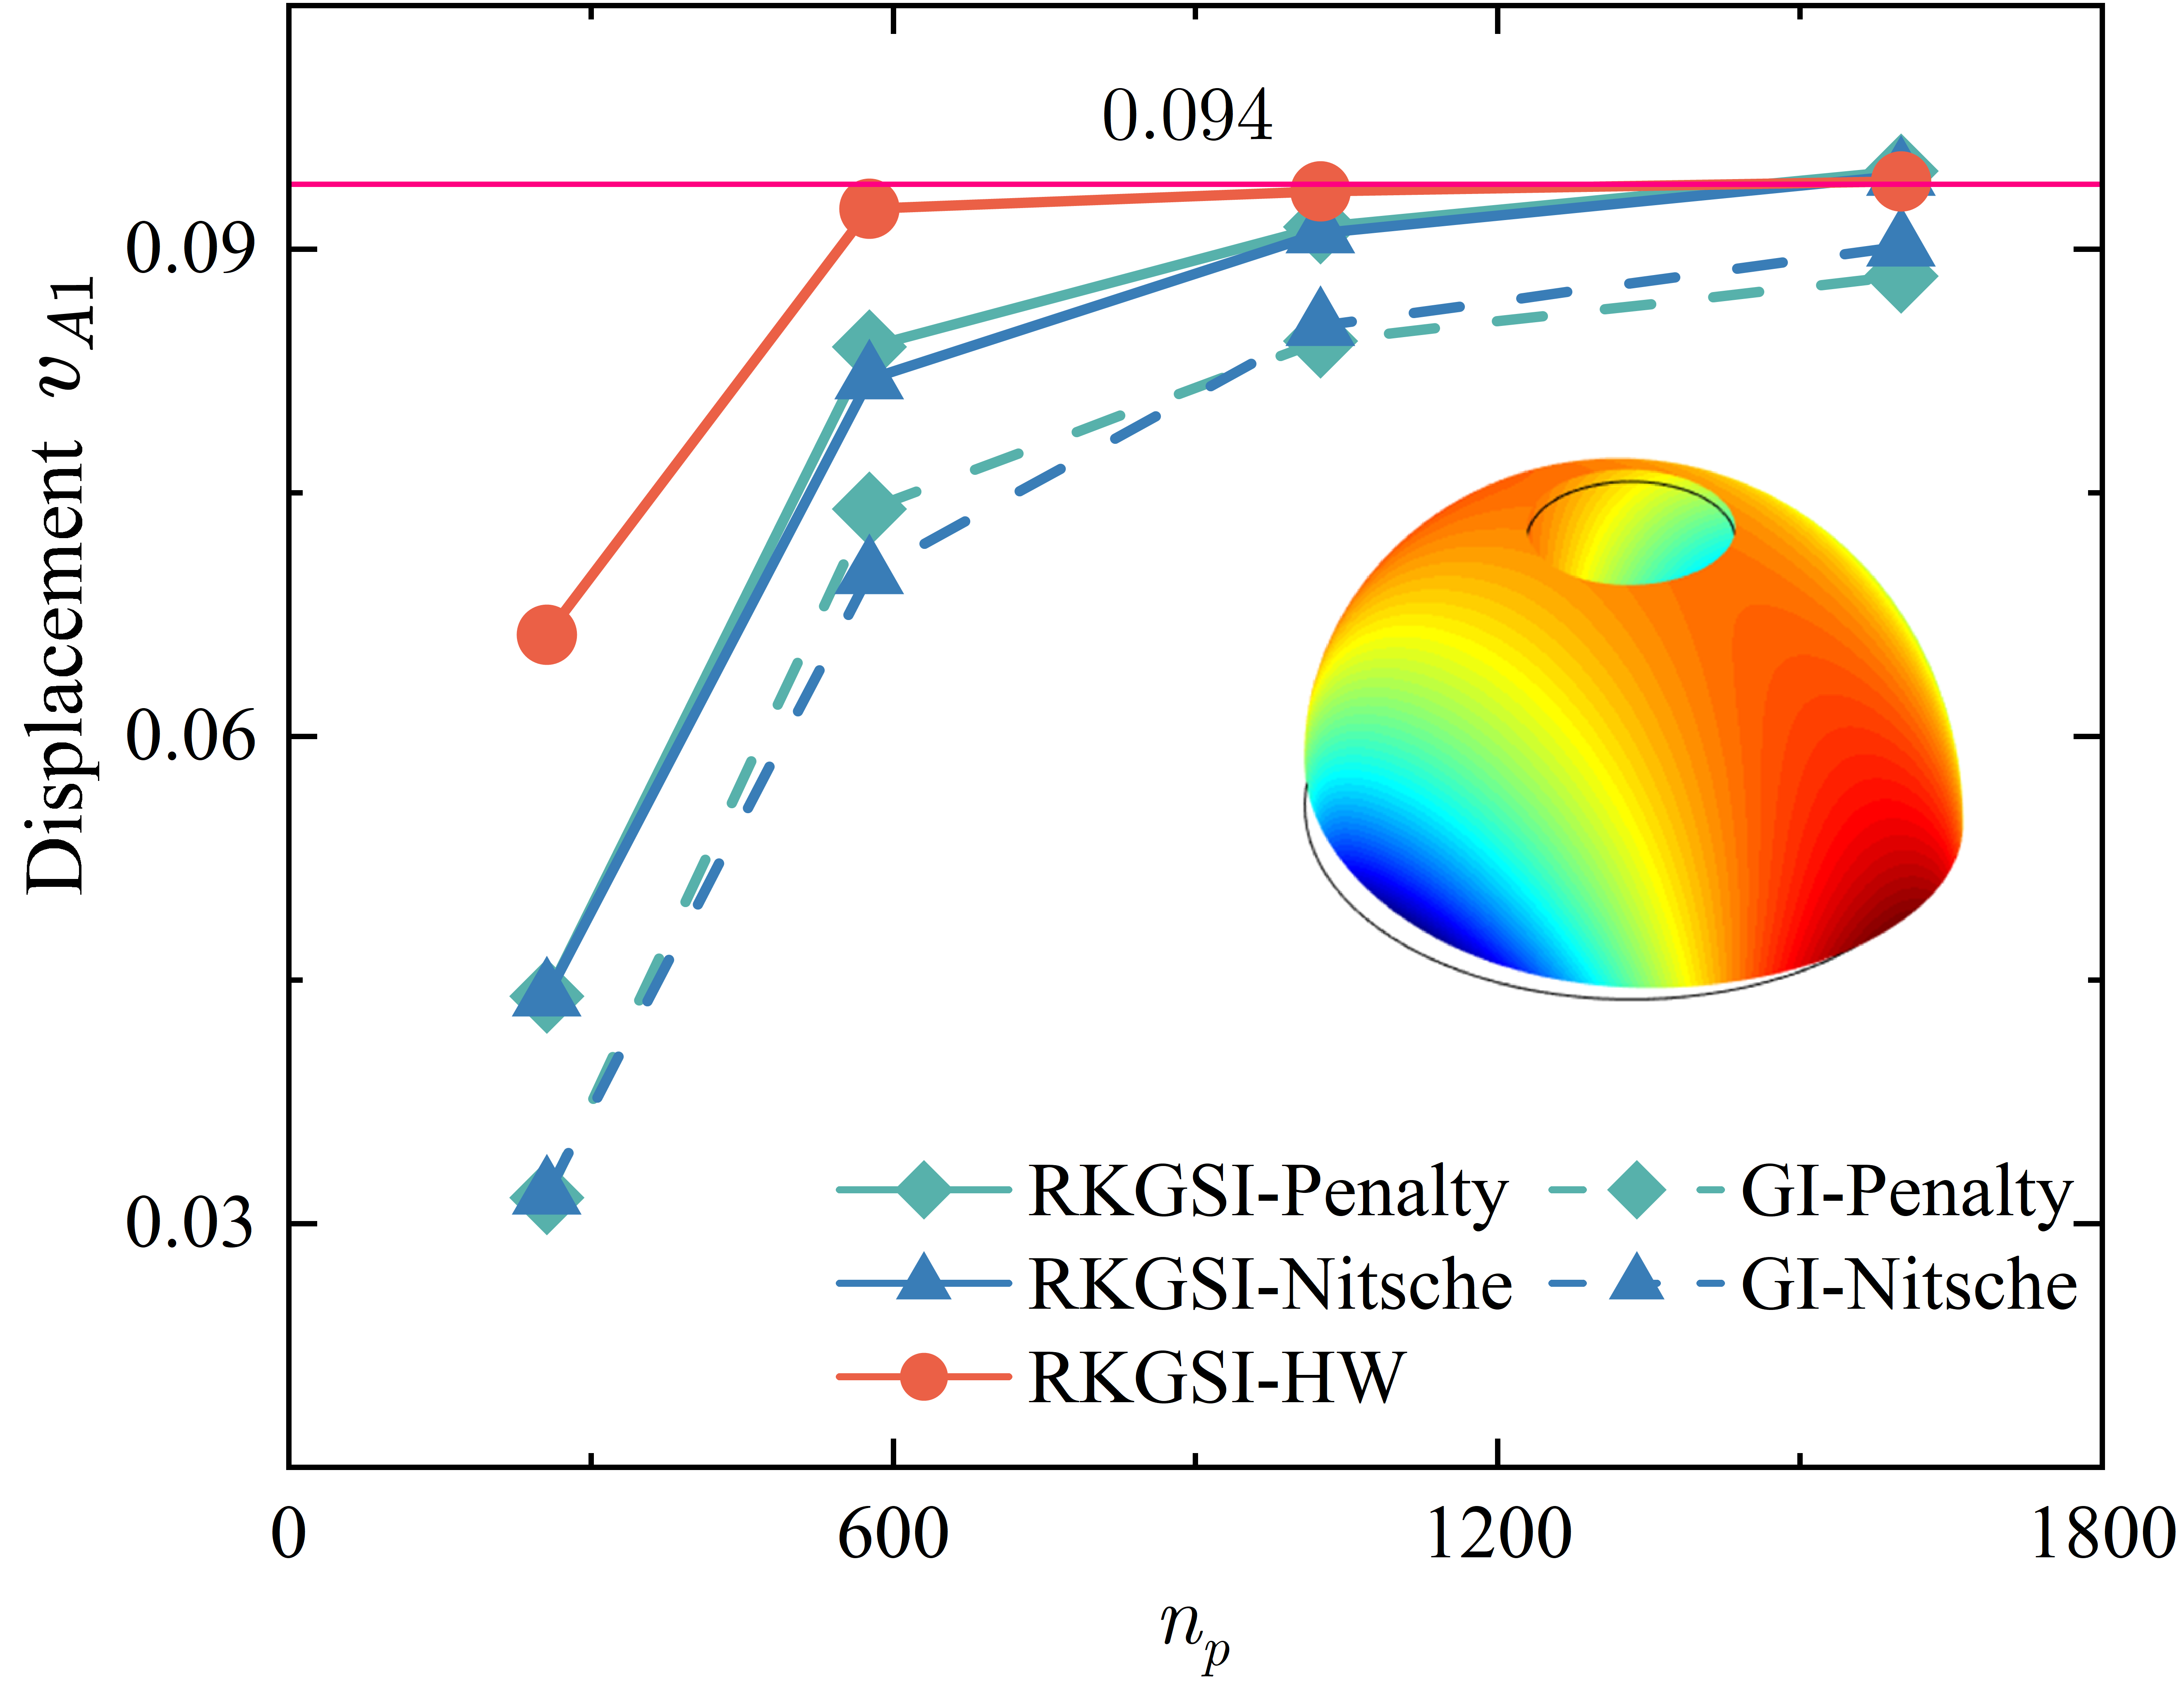
\includegraphics[height=0.7\textwidth]{figures/pfd_r1.png}
                \caption{球壳问题}
            \end{figure}
    \end{columns}
\end{frame}

\begin{frame}{数值算例}
    \begin{columns}
        \column{0.4\textwidth}
            \begin{figure}
                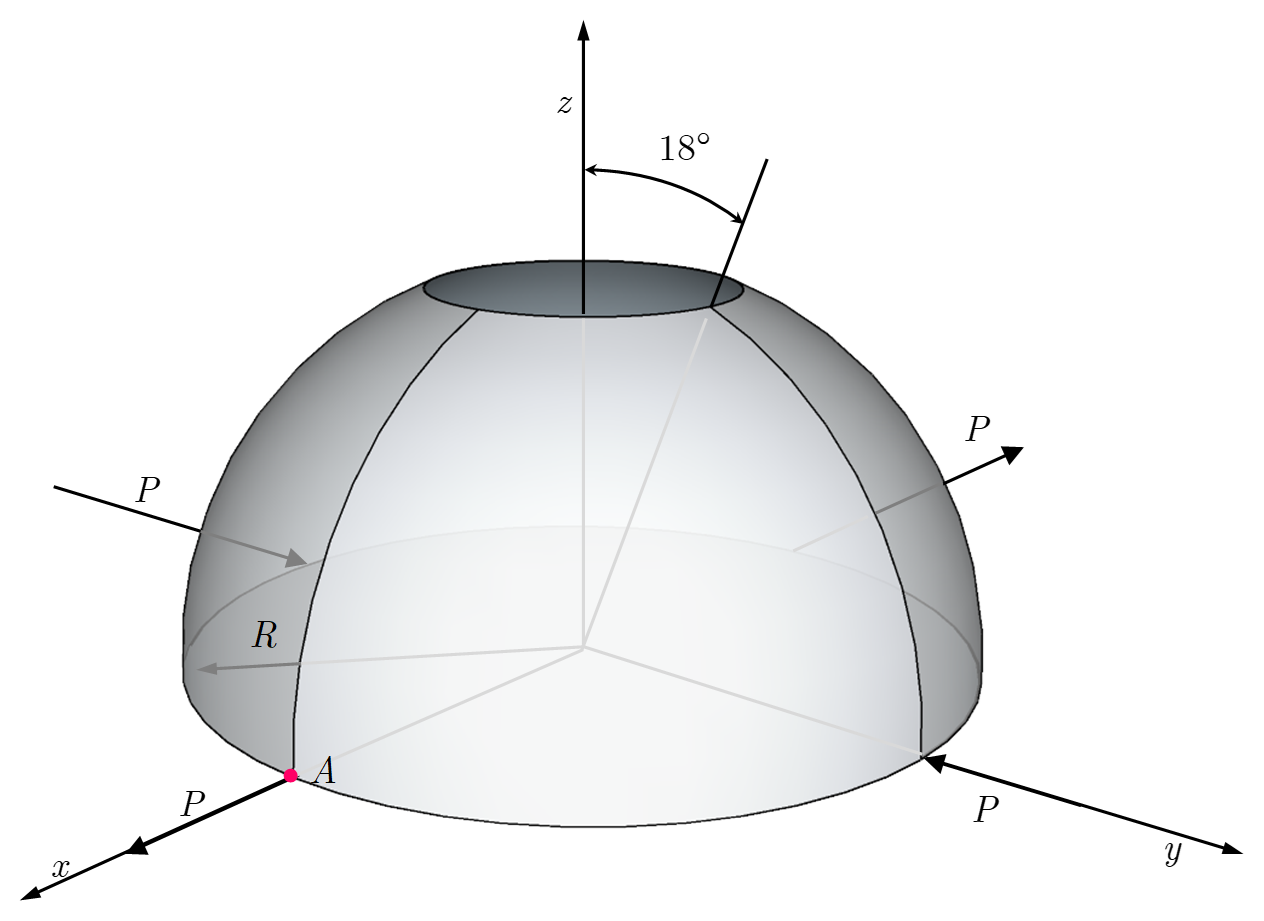
\includegraphics[width=\linewidth, trim=50 0 50 0, clip]{figures/pfm.png}
            \end{figure}
        \column{0.55\textwidth}
            \begin{figure}
                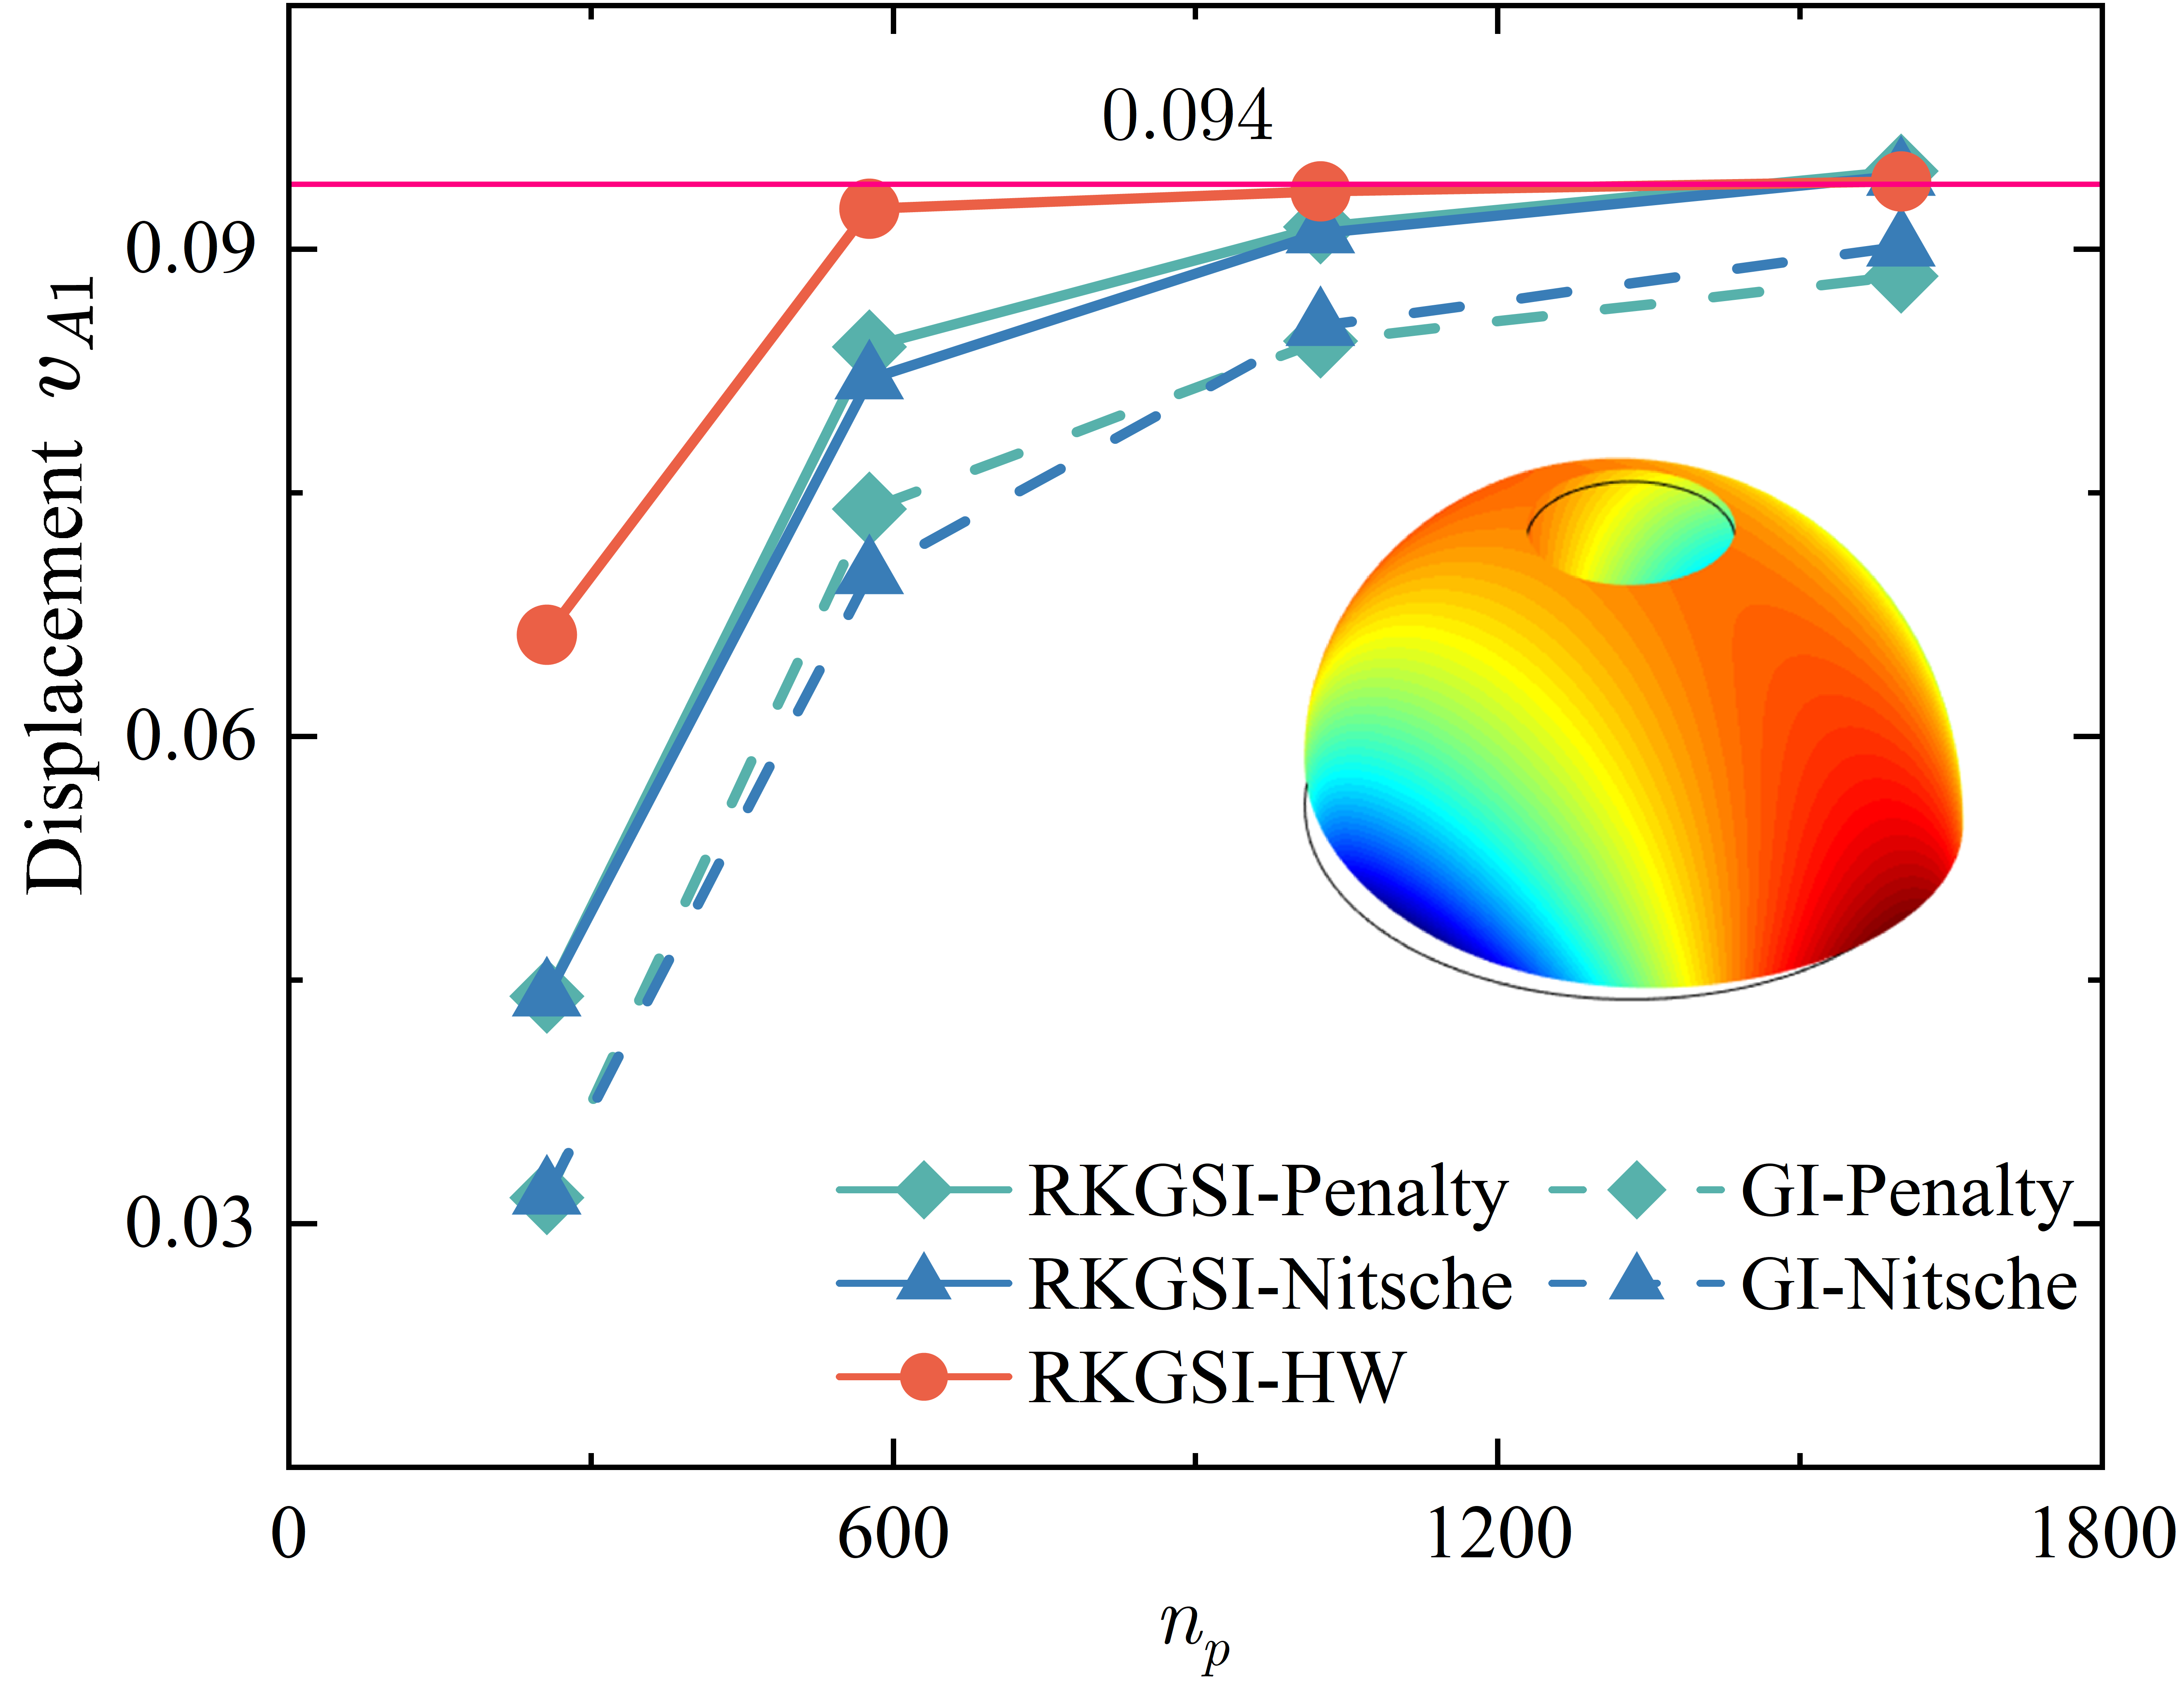
\includegraphics[height=0.7\textwidth]{figures/pfd_r1.png}
            \end{figure}
    \end{columns}

    \vspace{0.1cm}
    \centering
    \footnotesize
    \text{球壳问题}
\end{frame}

\begin{frame}{数值算例}
\begin{figure}[htbp]
    \centering 
    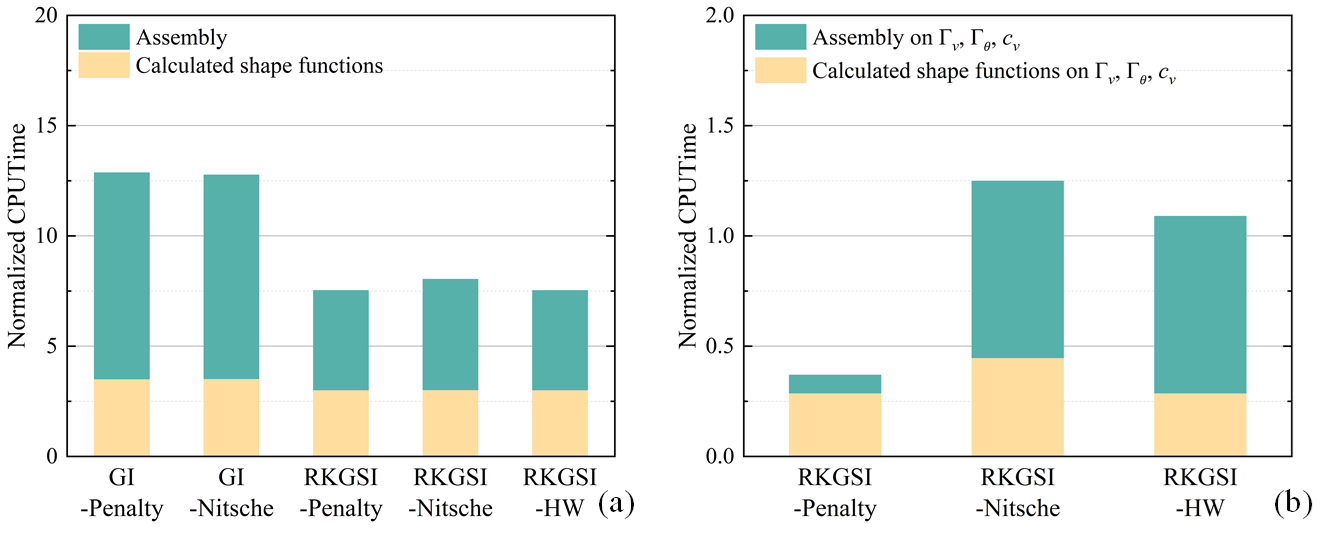
\includegraphics[width=0.95\textwidth]{figures/efficient.png}
    \caption{受压半球壳问题之效率比较：(a) 全域；(b) 本质边界}
\end{figure}
\end{frame}